\section{Chase-Lev Work-Stealing Deque}

\def\model{%
  \l{\textcolor{color1}{model}}%
}
\def\inv{%
  \l{\textcolor{color2}{inv}}%
}
\def\owner{%
  \l{\textcolor{color3}{owner}}%
}
\def\obligation{%
  \l{\textcolor{color4}{obligation}}%
}
\def\consumer{%
  \l{\textcolor{color5}{consumer}}%
}
\def\finished{%
  \l{\textcolor{color6}{finished}}%
}

\begin{frame}{Work-Stealing Deque}
\centering
\input{figures/work_stealing}
\end{frame}

\begin{frame}{Chase-Lev Work-Stealing Deque}
\centering
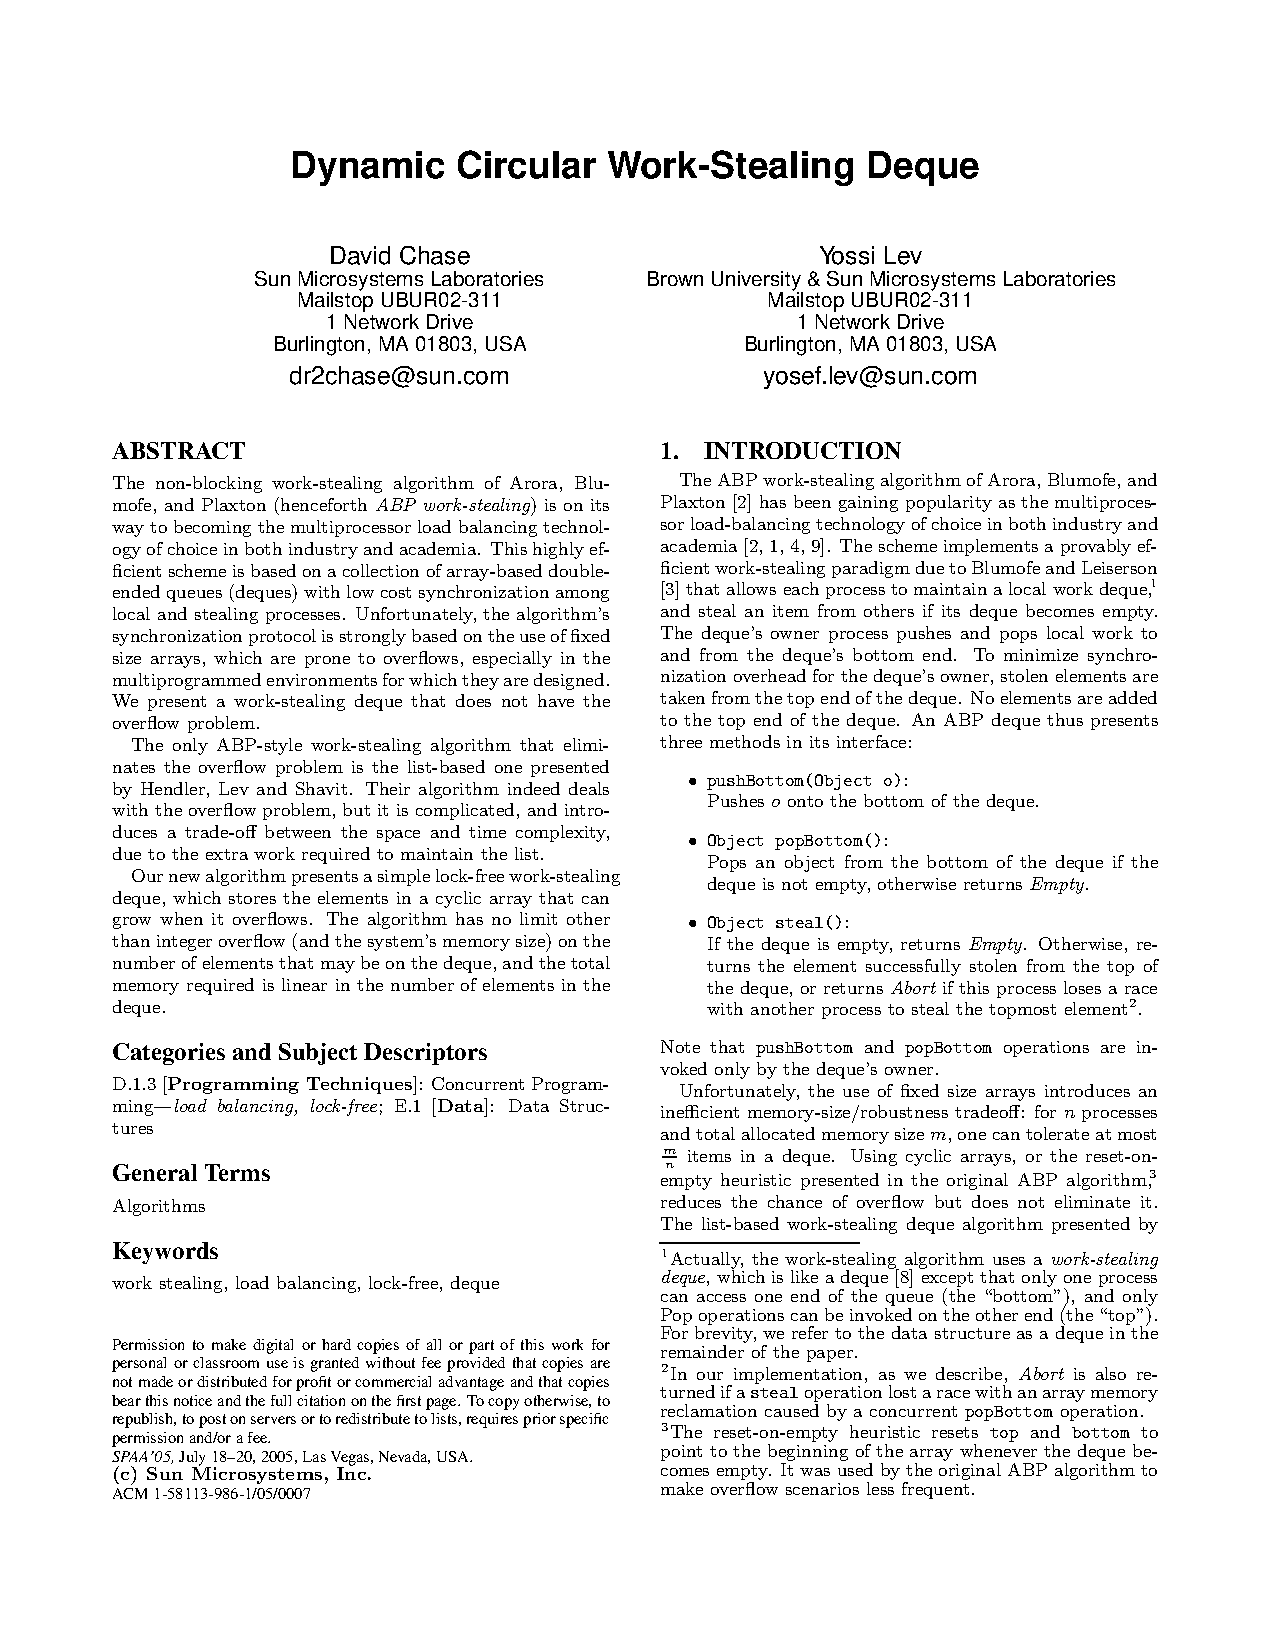
\includegraphics[scale=.5]{images/chaselev_paper.pdf}
\end{frame}

\begin{frame}{Déjà-Vu}
\centering
\only<1>{
  
\includegraphics[scale=.75, cframe=color2]{images/iris_workshop_2023_1.pdf}
}
\only<2>{
  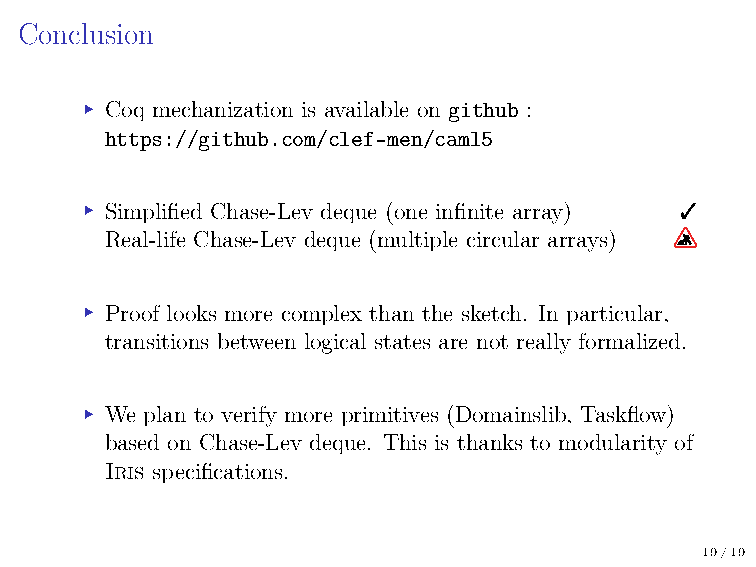
\includegraphics[scale=.75, cframe=color2]{images/iris_workshop_2023_2.pdf}
}
\end{frame}

\begin{frame}{My First Interaction With Robbert Krebbers}
\Large
\hfill
\begin{minipage}{.2\textwidth}

\includegraphics[scale=.15]{images/robbert_krebbers.jpg}
\end{minipage}
\hfill
\begin{minipage}{.7\textwidth}
\begin{quote}
  {
    Already verified in \c{iris/examples} \\
    \textcolor{color2}{without prophecy variables}! 
  } \\
  \\
  {
    \normalfont
    \large
    \textcolor{gray}{Robbert Krebbers, Iris Workshop 2023}
  }
\end{quote}
\end{minipage}
\hfill
\end{frame}

\begin{frame}{Future-Dependent Linearization Point}
\centering
\strut
\vfill
\input{figures/chaselev_logical_state}
\end{frame}

\begin{frame}{Weak Specification}
\begin{mathparpagebreakable}
    \iAspec[
      lab=steal-spec-weak
    ]{
      \inv\ t
    }[
      \zooVals
    ]{
      \model\ t\ \zooVals
    }{
      \c{steal}\ t
    }[
      o
    ]{
      \matchOption{
        o
      }{
        \model\ t\ \zooVals
      }{
        \zooVal
      }{
        \Exists \zooVals'. \\
        \zooVals = \cons{\zooVal}{\zooVals'} \iSep \\
        \model\ t\ \zooVals'
      }
    }[
      \v{res}
    ]{
      \v{res} = o
    }
  \and
    \iAspec[
      lab=pop-spec-weak
    ]{
      \inv\ t \iSep \\
      \owner\ t
    }[
      \zooVals
    ]{
      \model\ t\ \zooVals
    }{
      \c{pop}\ t
    }[
      o
    ]{
      \matchOption{
        o
      }{
        \model\ t\ \zooVals
      }{
        \zooVal
      }{
        \Exists \zooVals'. \\
        \zooVals = \zooVals' \dplus [\zooVal] \iSep \\
        \model\ t\ \zooVals'
      }
    }[
      \v{res}
    ]{
      \v{res} = o \iSep \\
      \owner\ t
    }
\end{mathparpagebreakable}
\begin{overbox}<2>
  \large
  \textbf{This specification is \emph{too weak} to prove completion :} \\
  Once the scheduler terminates, all submitted tasks have finished.
  \medskip
  \begin{mathpar}
      \infer[obligation-finished]{
          \obligation\ \v{pool}\ \iProp
        \\\\
          \finished\ \v{pool}
      }{
        \iLater \iPersistently \iProp
      }
    \and
      \infer[consumer-finished]{
          \consumer\ \v{pool}\ \iProp
        \\\\
          \finished\ \v{pool}
      }{
        \iFupd \iProp
      }
  \end{mathpar}
\end{overbox}
\end{frame}

\begin{frame}{Strong Specification}
\begin{mathparpagebreakable}
    \iAspec[
      lab=steal-spec
    ]{
      \inv\ t
    }[
      \zooVals
    ]{
      \model\ t\ \zooVals
    }{
      \c{steal}\ t
    }{
      \model\ t\ (\l{tail}\ \zooVals)
    }[
      \v{res}
    ]{
      \v{res} = \l{head}\ \zooVals
    }
  \and
    \iAspec[
      lab=pop-spec
    ]{
      \inv\ t \iSep \\
      \owner\ t\ \zooValsTwo
    }[
      \zooVals
    ]{
      \model\ t\ \zooVals
    }{
      \c{pop}\ t
    }[
      o\ \zooValsTwo'
    ]{
      \matchOption{
        o
      }{
        \zooVals = \nil \iSep
        \zooValsTwo' = \nil \iSep \\
        \model\ t\ \nil
      }{
        \zooVal
      }{
        \Exists \zooVals'. \\
        \zooVals = \zooVals' \dplus [\zooVal] \iSep
        \zooValsTwo' = \zooVals' \iSep \\
        \model\ t\ \zooVals'
      }
    }[
      \v{res}
    ]{
      \v{res} = o \iSep \\
      \owner\ t\ \zooValsTwo'
    }
\end{mathparpagebreakable}
\begin{overbox}<2>
  \large
  \textbf{This specification is \emph{sufficient} to prove completion :} \\
  Once the scheduler terminates, all submitted tasks have finished.
\end{overbox}
\end{frame}

\begin{frame}{Prophecy Variables / Prophets}
\large
\begin{itemize}
  \setlength\itemsep{1em}
  \item
    \textbf{Primitive prophets} \\
    Predict the future of the execution.
  \item
    \textbf{Typed prophets} \\
    Prediction belongs to a user-supplied semantic type.
  \item
    \textbf{\textcolor{color2}{Wise prophets}} \\
    Remember past predictions. \\
    Eliminate inconsistent branches.
  \item
    \textbf{\textcolor{color2}{Multiplexed prophets}} \\
    Separate logically independent predictions on a single prophet.
\end{itemize}
\end{frame}

% appear in other algorithms : array-based queue with impatient consumers, MemSnap algorithm
\begin{frame}{Multiplexed Prophets}
\def\model{%
  \l{\textcolor{color1}{model}}%
}
\def\snapshot{%
  \l{\textcolor{color3}{snapshot}}%
}
\def\key{%
  \textcolor{color2}{k}%
}
\begin{mathparpagebreakable}
    \infer[snapshot-get]{
      \model\ \zooProph\ \iGname\ \v{pasts}\ \v{prophss}
    }{
      \snapshot\ \iGname\ \key\ (\v{pasts}\ \key)\ (\v{prophss}\ \key)
    }
  \and
    \infer[snapshot-valid]{
        \model\ \zooProph\ \iGname\ \v{pasts}\ \v{prophss}
      \\
        \snapshot\ \iGname\ \key\ \v{past}\ \v{prophs}
    }{
      \Exists \v{past'}.
      \v{pasts}\ \key = \v{past} \dplus \v{past'} \iSep
      \v{prophs} = \v{past'} \dplus \v{prophss}\ \key
    }
  \\
    \infer[resolve-spec]{
        \iAtomic{\zooExpr}
      \\
        \l{to-val}\ \zooExpr = \None
      \\
        \zooVal = \recordGet{\v{prophet}}{to-val}\ \v{proph}
      \\
        \model\ \zooProph\ \iGname\ \v{pasts}\ \v{prophss}
      \\
        \iWp[
          mask=\iMask
        ]{
          \zooExpr
        }[
          \zooValTwo
        ]{
          \Forall \v{prophs}. \\
          \v{prophss}\ \key = \cons{\v{proph}}{\v{prophs}} \iWand \\
          \model\ \zooProph\ \iGname\ (\mapAlter{(\cdot \dplus [\v{proph}])}{\key}{\v{pasts}})\ (\mapInsert{\key}{\v{prophs}}{\v{prophss}}) \iWand \\
          \iPred\ \zooValTwo
        }
    }{
      \iWp[
        mask=\iMask
      ]{
        \zooExprResolve{\zooExpr}{\zooProph}{(\key, \zooVal)}
      }{
        \iPred
      }
    }
\end{mathparpagebreakable}
\end{frame}
